\documentclass[11pt,a4paper,oneside]{article}
\usepackage[dvipsnames, svgnames, x11names]{xcolor}
\usepackage{euler,amsthm,amsmath,amsfonts,graphicx,epigraph,indentfirst,enumerate,comment,listings,fontspec,color,subcaption,listings}
\usepackage{xeCJK}
\usepackage{hw}
\usepackage{pythonhighlight}
\usepackage{tikz}
\usepackage{algorithm}
\usepackage{algpseudocode}
\usepackage{float}

\newcommand{\nth}[1]{#1\textsuperscript{th}}
\newcommand{\E}{\mathop{\mathbb{E\/}}}
\newcommand{\N}{\mathbb{N}}
\newcommand{\R}{\mathbb{R}}

\renewcommand{\hwtitle} {CS217 Homework 3, First Submission}	
\renewcommand{\hwauthor}{Akina}
\renewcommand{\hwdate}{\today}

\begin{document}
\title{\hwtitle}
\author{\hwauthor}
\date{\hwdate}
\maketitle

\section*{Minimum Spanning Trees}

Throughout this assignment, let $G$ be a weighted graph, i.e., $G=(V,E,w)$ 
with $w: E \rightarrow \R^+$.
For $c \in \R$ and a weighted graph $G = (V,E,w)$, let
$G_c := (V, \{e \in E \ | \ w(e) \leq c\})$. That is, $G_c$ is the
subgraph of $G$ consisting of all edges of weight at most $c$.

\begin{problem}{1}
	\statement
	Let $T$ be a minimum spanning tree of $G$, and let $c \in \R$.  Show that
	$T_c$ and $G_c$ have exactly the same connected components.  (That
	is, two vertices $u,v \in V$ are connected in $T_c$ if and only if
	they are connected in $G_c$).
	You are encouraged to draw pictures to illustrate your proof!
	\solution
	
	\begin{proof}
		Since \(T_c\) is a subgraph of \(T\) consisting of all edges of weight at most \(c\) and \(T \subseteq G\), we have  \(T_c = T \cap G_c\). This implies that \(T_c \subseteq G_c\). Hence, if two vertices \(u, v\) are connected in \(T_c\), they are connected in \(G_c\). Hence the number of the connected components of \(T_c\) less than or equal to the number of \(G_c\)
		
		If we add edges in \(G_c / T_c\) one by one to \(T_c\), we finally get \(G_c\). Assume that \(T_c\) and \(G_c\) have different connected components, there must exist a edge, it connects two different components of \(T_c\), denoted by \(\{u, v\}\). Consider the path \(P: u(p_1), p_2, p_3, \dots, p_{k-1}, v(p_k)\) in \(T\), there must exist \(1 \leq i < k\), such that \(\{p_i, p_{i+1} \} \not\in T_c\), then \(w(\{p_i, p_{i+1}\}) > c\). If we replace \(\{p_i, p_{i+1}\}\) with \(e\), we will get another spanning tree with cheaper weight sum. A contradiction.
		
		Hence, \(T_c\) and \(G_c\) have exactly the same connected components.
	\end{proof}
\end{problem}

\begin{problem}{2}
	\statement
	For a weighted graph $G$, let $m_c(G) := | \{ e \in E(G) \ | \ w(e) \leq c\}|$, i.e.,
	the number of edges of weight at most $c$ (so $G_c$ has $m_c(G)$ edges).
	Let $T, T'$ be two minimum spanning trees of $G$. Show that
	$m_c(T) = m_c(T')$.

	\solution
	
	We prove it by reduction to absurdity. Without loss of generality, let \(m_c(T) > m_c(T')\). According to \textbf{Problem 1} we know, both \(T_c\) and \(T'_c\) have the same connected components as \(G_c\), hence \(T_c\) and \(T'_c\) have the same connected components. There must exist a connected components, which contains more edges in \(T_c\) than \(T'_c\). \(T'\) does not contain circles, hence so does \(T'_c\) since it is a subgraph of \(T'\). So \(T'_c\) is a tree. If \(T_c\) has more edges than a tree, it must contain circle. A contradiction.
	
	Hence \(m_c(T) = m_c(T')\).
	
\end{problem}
\begin{problem}{3}
	\statement
	Suppose $G$ is connected, and no two edges of $G$ have the same weight. 
	Show that $G$ has exactly one minimum spanning tree!
	
	\solution  
	
	Assume that \(G\) has two different minimum spanning trees, denoted by \(T\) and \(T'\). There exist an edge \(e = \{u, v\}\), such that \(e \in T\) but \(e \not\in T'\). Consider the path \(P: u(p_1), p_2, p_3, \dots, p_{k-1}, v(p_k)\) in \(T'\). because \(T_{w(e)}\) and \(T'_{w(e)}\) have the same connected components, each edge in \(P\) has a weight cheaper than or equal to \(w(e)\), otherwise \(u\) and \(v\) will be disconnected. because no two edges of \(G\) have the same weight, then \(w(\{p_i, p_{i+1}\} < w(e) (1 \leq i < k)\). We can repalce \(e \in T\) with any edge in path \(P\) to get another spanning tree with cheaper weight sum. A contradiction.
	
	Hence, \(G\) has exactly one minimum spanning tree.
\end{problem}

\section*{}
A {\em multigraph} is a graph that can have multiple edges, called
``parallel edges''. Without defining 
it formally, we illustrate it:
\begin{center}
	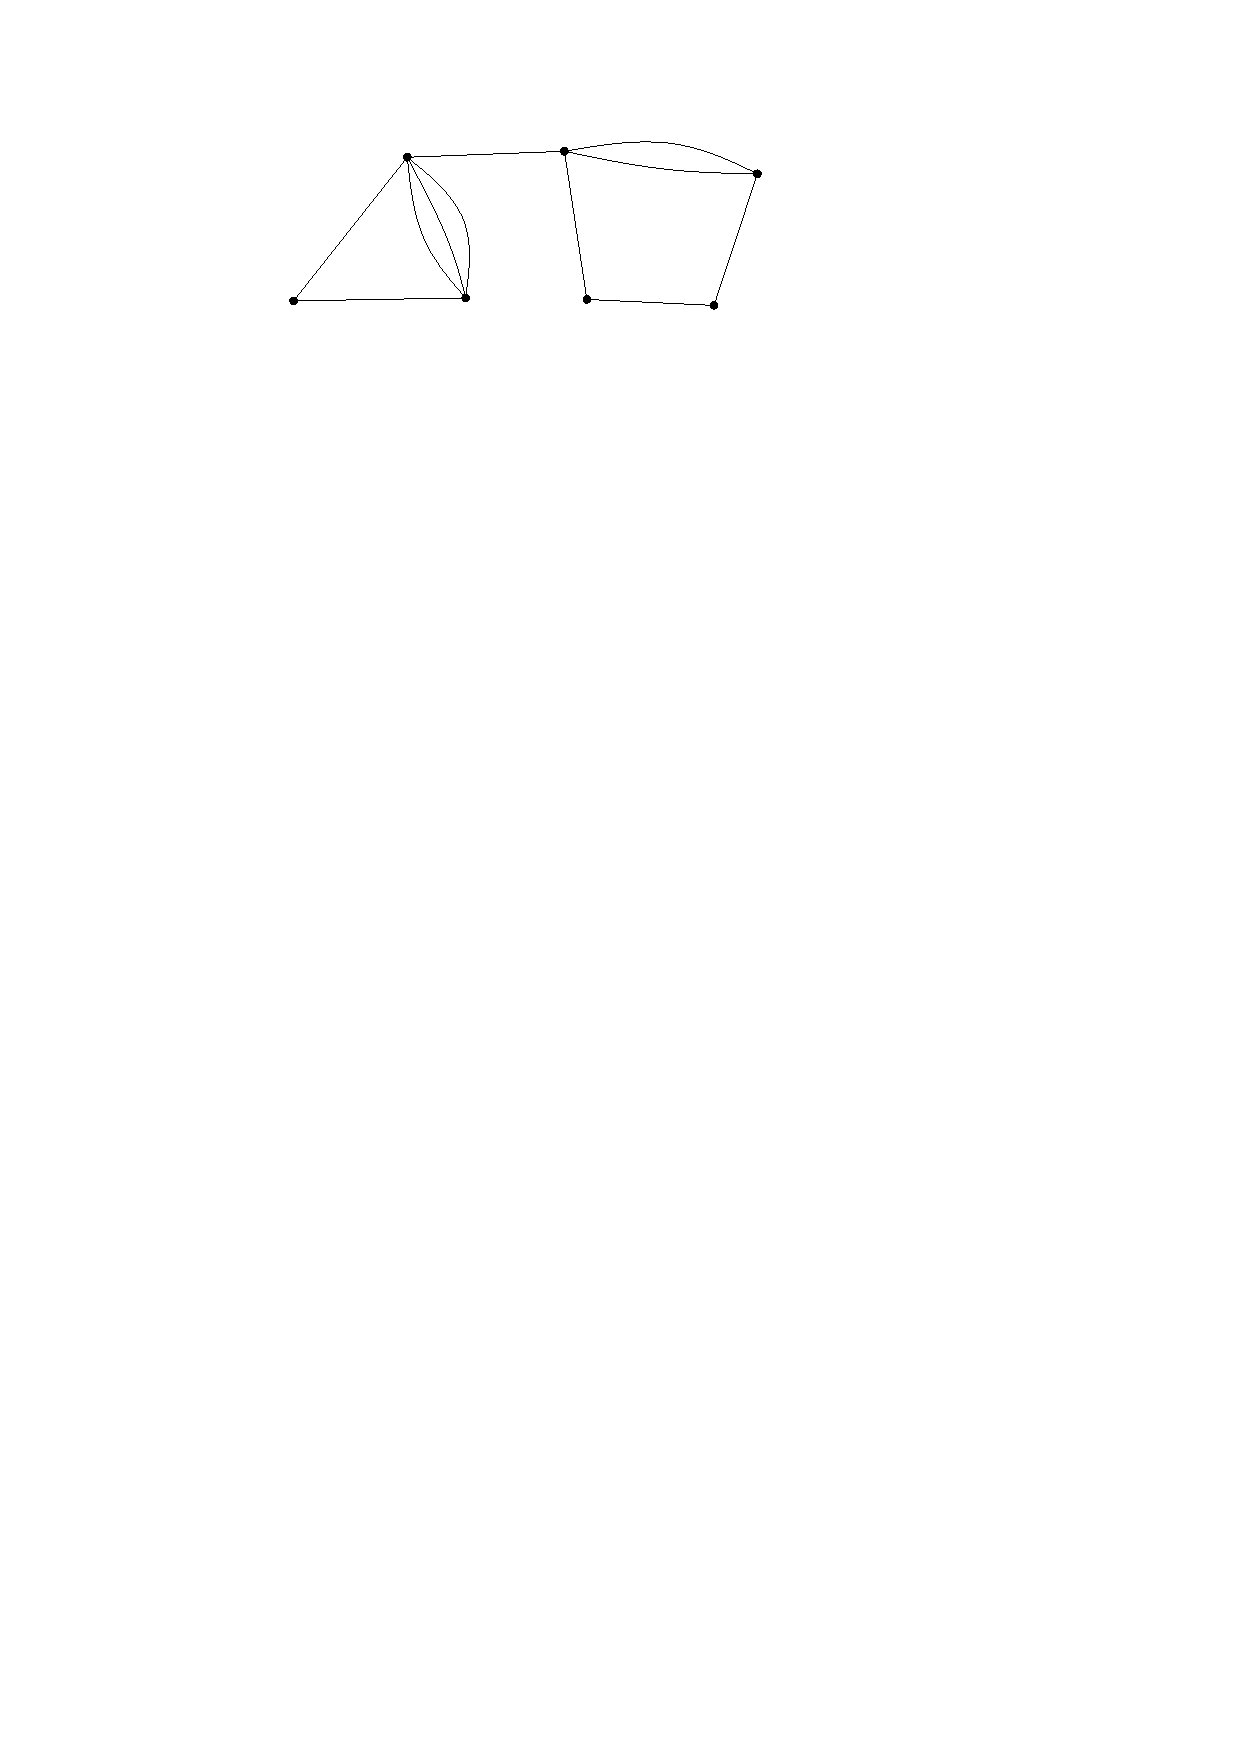
\includegraphics[width=0.6\textwidth]{figures/multigraph.pdf}\\
	A multigraph.
\end{center}
All other definitions, like connected components and spanning trees
are the same as for normal (simple) graphs. However,
when two spanning trees use different parallel edges, we consider them
different:
\begin{center}
	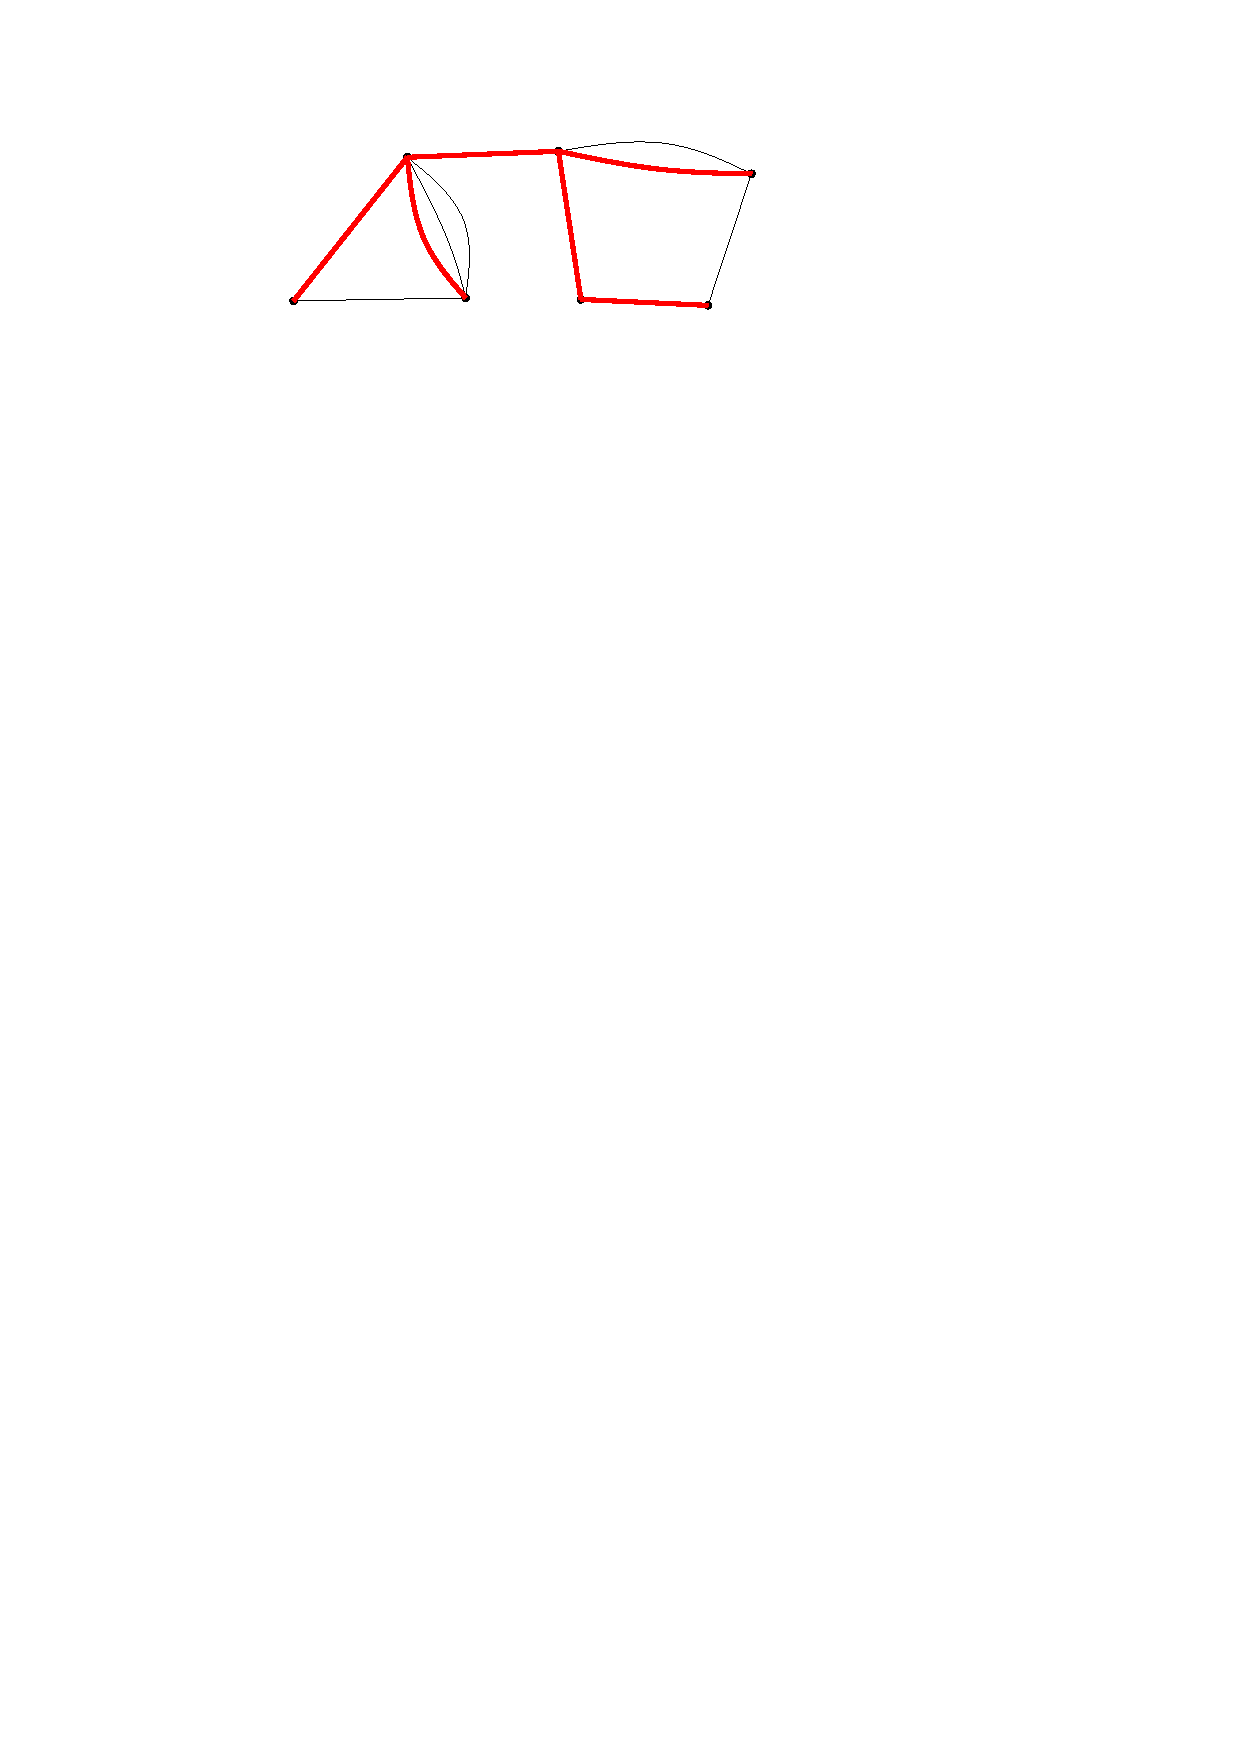
\includegraphics[width=0.4\textwidth]{figures/multigraph-forest.pdf} \hspace{2cm}
	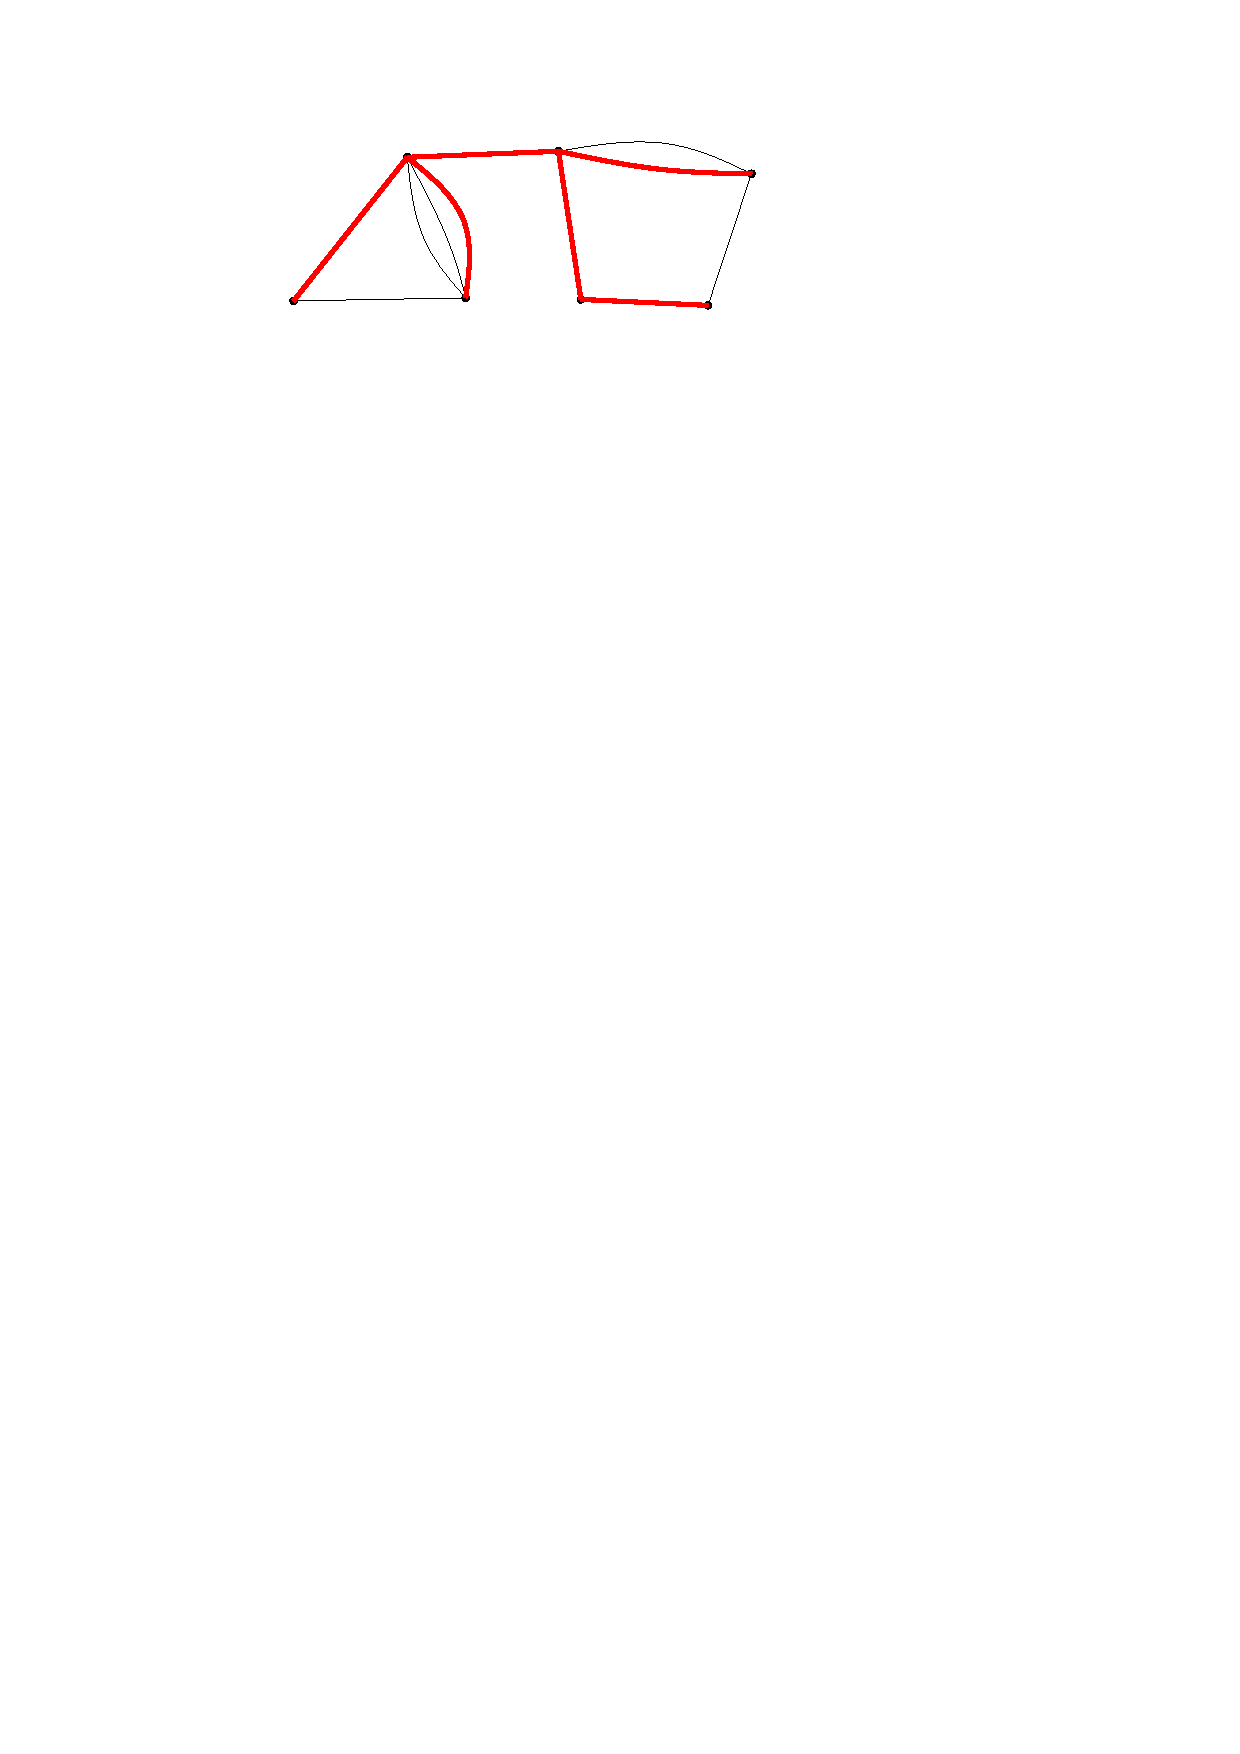
\includegraphics[width=0.4\textwidth]{figures/multigraph-forest-other.pdf} \\
	The same multigraph with two different spanning trees.
\end{center}

\begin{problem}{4}
\statement
How many spanning trees does the above multigraph on 7 vertices have?
Justify your \text{answer}!

\solution

$49$. We will give two proofs.
\begin{proof}
Observe the multigraph: First we consider both the multiedges as simple edges, then the graph is a triangle and a quadrangle connected by a bridge. The bridge must be chosen. In triangle, there are $1 + 2 \times 3$ ways to form a tree. In quadrangle, there are $1 + 3 \times 2$ ways. Simply multiply them, therefore the \text{answer} is $49$.
\end{proof}
\begin{proof}
Using Kirchhoff's theorem we can justify our \text{answer} simply calculate the determinant of Laplacian matrix for the multigraph. Using the following code
\begin{python}
import numpy as np
n, m = map(int, input().split())
K = np.zeros((n, n), dtype=np.int64)
for i in range(m):
	u, v = map(lambda x:int(x) - 1, input().split())
	K[u][u] -= 1
	K[v][v] -= 1
	K[u][v] += 1
	K[v][u] += 1
K = np.delete(K, 0, 0)
K = np.delete(K, 0, 1)
print(int(round(np.linalg.det(K))))
\end{python}
and input data
\begin{python}
7 11
1 2
1 3
2 3
2 3
2 3
2 4
4 5
5 6
6 7
4 7
4 7
\end{python}
Then we get \text{answer}
\begin{python}
49
\end{python}
\end{proof}
\end{problem}

\begin{problem}{5}
\statement
Suppose you have a polynomial-time algorithm that, given a multigraph $H$,
computes the number of spanning trees of $H$.
Using this algorithm as a subroutine, design a polynomial-time algorithm
that, given a weighted graph $G$, computes the number of 
minimum spanning trees of $G$.

\solution

We use denote the union find set as $UFset$, and the polynomial­-time algorithm to count trees as \textsc{CountTree}. In order to keep the pseudocode simple, there are many set operations used in the code that should be implemented with sortings, taggings, and traversings. With best implementation it should be $O(m \log m + n ^ 3)$, assuming that the polynomial­-time algorithm is based on Kirchhoff's Matrix Tree theorem and Gauss elimination.

\begin{algorithm}
	\caption{Computes number of MST in $G$}
	\begin{algorithmic}[1]
		\Procedure{CountMST}{$V, E$}
		\State $UFset.\text{initialize}(|V|)$
		\State $ans \gets 1$
		\For{$w \in w(E)$ increasingly}
		\State $E_w \gets \big\{e \in E \big| w(e) = w\big\}$
		\State $UFset_w \gets UFset.\text{union}(E_w)$
		\State $V_w \gets \big\{UFset_w.\text{find}(v) \big| v \in V \big\}$
			\For{$c \in V_w$} 
				\State $V' \gets \big\{UFset.\text{find}(v) \big| UFset_w.\text{find}(v) = c, v \in V\big\}$
				\State $E' \gets \big\{ \{UFset.\text{find}(u), UFset.\text{find}(v)\} \big| UFset_w.\text{find}(u) = UFset_w.\text{find}(v) = c, \{u, v\} \in E_w\big\}$
				\State $ans \gets ans \times \textsc{CountTree}(V', E')$
			\EndFor
		\State $UFset \gets UFset_w$
		\EndFor
		\EndProcedure
	\end{algorithmic}
\end{algorithm}


\end{problem}

\end{document}
